\documentclass[a4paper, 12pt]{article}
% math symbols
\usepackage{amssymb}
\usepackage{amsmath}
\usepackage{mathrsfs}
\usepackage{physsummer}


\usepackage{enumitem}
\usepackage[margin = 2cm]{geometry}

\tolerance = 1000
\emergencystretch = 0.74cm



\pagestyle{empty}
\parindent = 0mm

\setphysstyle{ГЦФО 10}{Вступительная олимпиада}{06.09.2016}

\begin{document}

\large

\taskpic{ В гладкой закрепленной полусфере свободно лежит палочка
  массы $m$ так, что угол ее с горизонтом равен $\alpha$, а конец
  выходит за край полусферы. С какими силами действует палочка на
  полусферу в точках соприкосновения $A$ и $B$?}
{
  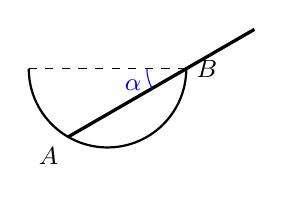
\begin{tikzpicture}\small
    \pgfmathsetmacro{\a}{60};
    \draw [thick] (0,0) arc (0 : -180 : 1);
    \draw [very thick] (90-\a : 1) -- (0,0) node [right=.1] {$B$} -- (
    {-1+cos(2*\a)}, {-sin(2*\a)})node[below left] {$A$};
    \draw [dashed] (0,0) -- (-2,0);
    \draw [blue] (270-\a : .5) arc (270-\a : 180 : .5) node [pos=.2,
    left] {$\alpha$};
  \end{tikzpicture}
}

\taskpic[6cm]{ Определите общее сопротивление между точками $A$ и $B$
  цепи, изображенной на рисунке. }
{
  \begin{tikzpicture}[circuit ee IEC, every resistor/.style = {circuit
      symbol size = width 2.5 height 1}, thick]\small
    \pgfmathsetmacro{\r}{1.2}
    \draw (0, .5*\r) to [resistor={info=$1~\Omega$}] ++ (\r,0) to
    [resistor={info=$2~\Omega$}] ++ (\r,0) to
    [resistor={info=$3~\Omega$}] ++ (\r,0);
    \draw (0, -.5*\r) to [resistor={info'=$3~\Omega$}] ++ (\r,0) to
    [resistor={info'=$2~\Omega$}] ++ (\r,0) to
    [resistor={info'=$1~\Omega$}] ++ (\r,0);
    \draw (1*\r, .5*\r) to [resistor={info'=$2~\Omega$}] ++ (0, -\r)
    (2*\r, .5*\r) to [resistor={info=$2~\Omega$}] ++ (0, -\r);
    \draw (0, -.5*\r) --++ (0, \r) (3*\r, -.5*\r) --++ (0, \r);
    \draw [*-] (-.5, 0) node [below] {$A$} -- (0,0);
    \draw [-*] (3*\r, 0) --++ (.5, 0) node [below] {$B$};
  \end{tikzpicture}
}

\task{ Частица массы $m_1$ налетела со скоростью $v$ на неподвижную
  частицу массы $m_2$, которая после упругого удара полетела под углом
  $\alpha$ к первоначальному направлению движения налетающей
  частицы. Определите скорость частицы массы $m_2$ после удара.  }

\taskpic{ Две материальные точки $1$ и $2$ и точечный источник света
  $S$ совершают равномерное прямолинейное движение по горизонтальной
  плоскости. Тени от материальных точек $1$ и $2$ движутся со
  скоростями $u$ вдоль вертикальных стенок, которые перпендикулярны
  друг другу. Скорости материальных точек равны $v=2u/\sqrt{3}$ и
  направлены под углом $\alpha=30^\circ$ к соответствующим стенкам
  (см. рисунок). Чему равна и куда направлена скорость источника S?}
{
  \begin{tikzpicture}[scale=1.3]\scriptsize
    \pgfmathsetmacro{\a}{30};
    \pgfmathsetmacro{\r}{1};
    \fill [pattern=north west lines] (-.15,-.15) rectangle (2,2);
    \fill [white] (0,0) rectangle (2.2, 2.2);
    \draw (2,0) -| (0,2);
    \draw [->, thick] (.3, .9) --++ (90-\a : \r );
    \draw [blue] (.3, .9 + .4) arc (90 : 90-\a : .4 ) node [pos=.7, above] {$\alpha$};
    \draw [blue] (.9 + .4, .3) arc (0 : \a : .4 ) node [pos=.7, right] {$\alpha$};
    \draw [->, thick] (.9, .3) --++ (\a : \r);
    \draw [dashed, blue] (.3, .9) --++ (0, {\r*cos(\a)} ) (.9, .3)
    --++ ( {\r*cos(\a)}, 0);
    \draw [dashed] (.9, 0) |- (0, .9);
    \draw [->, very thick] (0, .9) --++ ( 0, {\r*cos(\a)} );
    \draw [->, very thick] (.9, 0) --++ ( {\r*cos(\a)}, 0 );
    \filldraw [ thick, fill=white ] (.9, .9) circle (.04) node
    [right=.02] {$S$} ;
  \end{tikzpicture}
}


\end{document}


%%% Local Variables: 
%%% mode: latex
%%% TeX-engine:xetex
%%% TeX-PDF-mode: t
%%% End:
